\documentclass[12pt, a4paper]{report}
\usepackage{caption, subcaption}
\usepackage[utf8]{inputenc}
\usepackage[italian]{babel}
\usepackage[T1]{fontenc}
\usepackage{graphicx}
\usepackage[top=3cm, bottom=3cm]{geometry}
\usepackage{tabularx}
\usepackage{titlesec}
\usepackage{colortbl}
\usepackage{csquotes}
\usepackage{amsmath}
\usepackage{amssymb}
\usepackage{xcolor}
\usepackage{array}
\usepackage{float}

\newcommand{\apj}{\textit{The Astrophysical Journal}}
\newcommand{\mnras}{\textit{Monthly Notices of the Royal Astronomical Society}}
\newcommand{\aap}{\textit{Astronomy \& Astrophysics}}
\newcommand{\nar}{\textit{New Astronomy Reviews}}
\newcommand{\araa}{\textit{Annual Review of Astronomy and Astrophysics}}

\usepackage[backend=biber, style=authoryear]{biblatex}
\addbibresource{bibliografia.bib}

\newcolumntype{C}[1]{>{\centering\arraybackslash}p{#1}}

\renewcommand*{\nameyeardelim}{\addspace}
\renewcommand*{\postnotedelim}{\addcolon\space}
\renewcommand*{\finentrypunct}{)}
\renewcommand{\chaptername}{Capitolo}

\begin{document}

L'obiettivo del lavoro di tesi è valutare le dimensioni e le eccentricità dei dischi circumstellari in dipendenza dei parametri del sistema binario che li ospita.
L'analisi da noi effettuata si concentra sul mass-ratio $q$, sull'eccentricità $e$ della binaria e sulla viscosità del materiale costituente il disco.\\

\textbf{Disco protoplanetario}\\

I dischi proto-planetari sono delle strutture sottili costituite da gas e polveri che orbitano attorno ad una stella.
L'evoluzione del disco è dettata da fenomeni che compo

Le stelle si formano in dense nubi molecolari, che sono delle regioni di spazio ($\sim 10\,-\,100\,pc$) riempite di gas e polveri (massa $\sim 10^4\,-\,10^6\,M_\odot$). 
Alcune zone di queste nubi, dette \textit{cores}, sono gravitazionalmente instabili e presentano momento angolare non nullo \parencite{Goodman1993}: il loro collasso porta alla formazione di una nuova stella. 
Durante tale processo si viene a creare un disco sottile attorno alla proto-stella costituito da gas e polveri: questa struttura è detta \textit{disco protoplanetario}.
La vita media di un tale oggetto è $t \sim 10^6$ yr, poiché l'ultima fase della formazione stellare è caratterizzata da un graduale accrescimento di materiale sul corpo centrale: il processo è regolato da meccanismi che determinano una ridistribuzione del momento angolare.
I dischi d'accrescimento sono dinamicamente freddi: l'evoluzione è supersonica, ossia la velocità del suono $c_s$ è molto minore della velocità di rotazione $v_\varphi$.

L'esistenza di sistemi stellari multipli è una conseguenza naturale del processo di formazione stellare: il nostro lavoro è focalizzato sulla casistica binaria.
La presenza di più corpi influenza fortemente l'evoluzione dei singoli dischi d'accrescimento presenti: le forze di marea causate dalla presenza dei compagni portano al troncamento dei dischi proto-planetari.
Una binaria \textit{pre-main sequence} può presentare tre dischi protoplanetari distinti: due circumstellari ed uno circumbinario.
L'estensione degli stessi è dettata dalle interazioni dinamiche fra stelle e materiale orbitante: il raggio di troncamento $r_T$ dipende dall'eccentricità $e$ dell'orbita del sistema binario, dal mass-ratio $q$, dalla viscosità $\alpha$ e dalla temperatura $T$ del disco (\cite{PapaloizouPringle1977}; \cite{ArtymowiczLubow1994}; \cite{Pichardo2005}).

Il lavoro di tesi ha come obiettivo lo studio numerico delle dimensioni e delle eccentricità caratteristiche dei dischi circumstellari al variare di $e$, $q$ ed $\alpha$. Abbiamo deciso di valutare la dipendenza dalla viscosità del materiale lavorando con $\alpha\,\in\,\{10^{-2},\, 10^{-3},\,10^{-4}\}$, in modo tale da esplorare l'intervallo caratteristico dei dischi proto-planetari.
I sistemi binari che abbiamo analizzato possono essere divisi in tre categorie: circolari ($e\,=\,0.0$), a media eccentricità ($e\,=\,0.3$) e ad elevata eccentricità ($e\,=\,0.6$).
Abbiamo studiato quattro rapporti fra la massa $m_2$ della stella secondaria e quella $m_1$ della primaria: $m_2/m_1\,=\,0.1,\,0.33,\,0.5,\,1$.

Per effettuare le simulazioni abbiamo utilizzato FARGO3D, che è un codice magneto-idrodinamico sviluppato con l'obiettivo di studiare la fisica dei dischi proto-planetari. FARGO3D risolve le equazioni differenziali caratteristiche del problema in analisi su una griglia euleriana lavorando con metodi alle differenze finite ed ai volumi finiti.
La risoluzione con cui abbiamo lavorato è di 384 celle radiali $n_r$ e 1152 celle azimutali $n_\varphi$. 
Il sistema viene inizializzato specializzando il profilo di densità del gas in modo tale che sia presente un quantitativo maggiore di materiale a piccoli raggi e viene fatto evolvere per cinquanta orbite del sistema binario: ogni mezzo periodo di rivoluzione viene effettuato un output.
Le dimensioni del disco e la sua eccentricità vengono valutate per ogni configurazione assunta dal materiale fra il trentesimo e il cinquantesimo periodo: i risultati che forniamo sono i valori medi delle stime effettuate. Abbiamo determinato l'estensione dei dischi con due metodi differenti: per ogni sistema in analisi effettuiamo una stima del raggio di troncamento e del semiasse maggiore del disco. In Figura \ref{fig:sax_magg} sono riportati i valori di semiasse maggiore ottenuti per le tre viscosità considerate.

\begin{figure}[H]
    \centering
    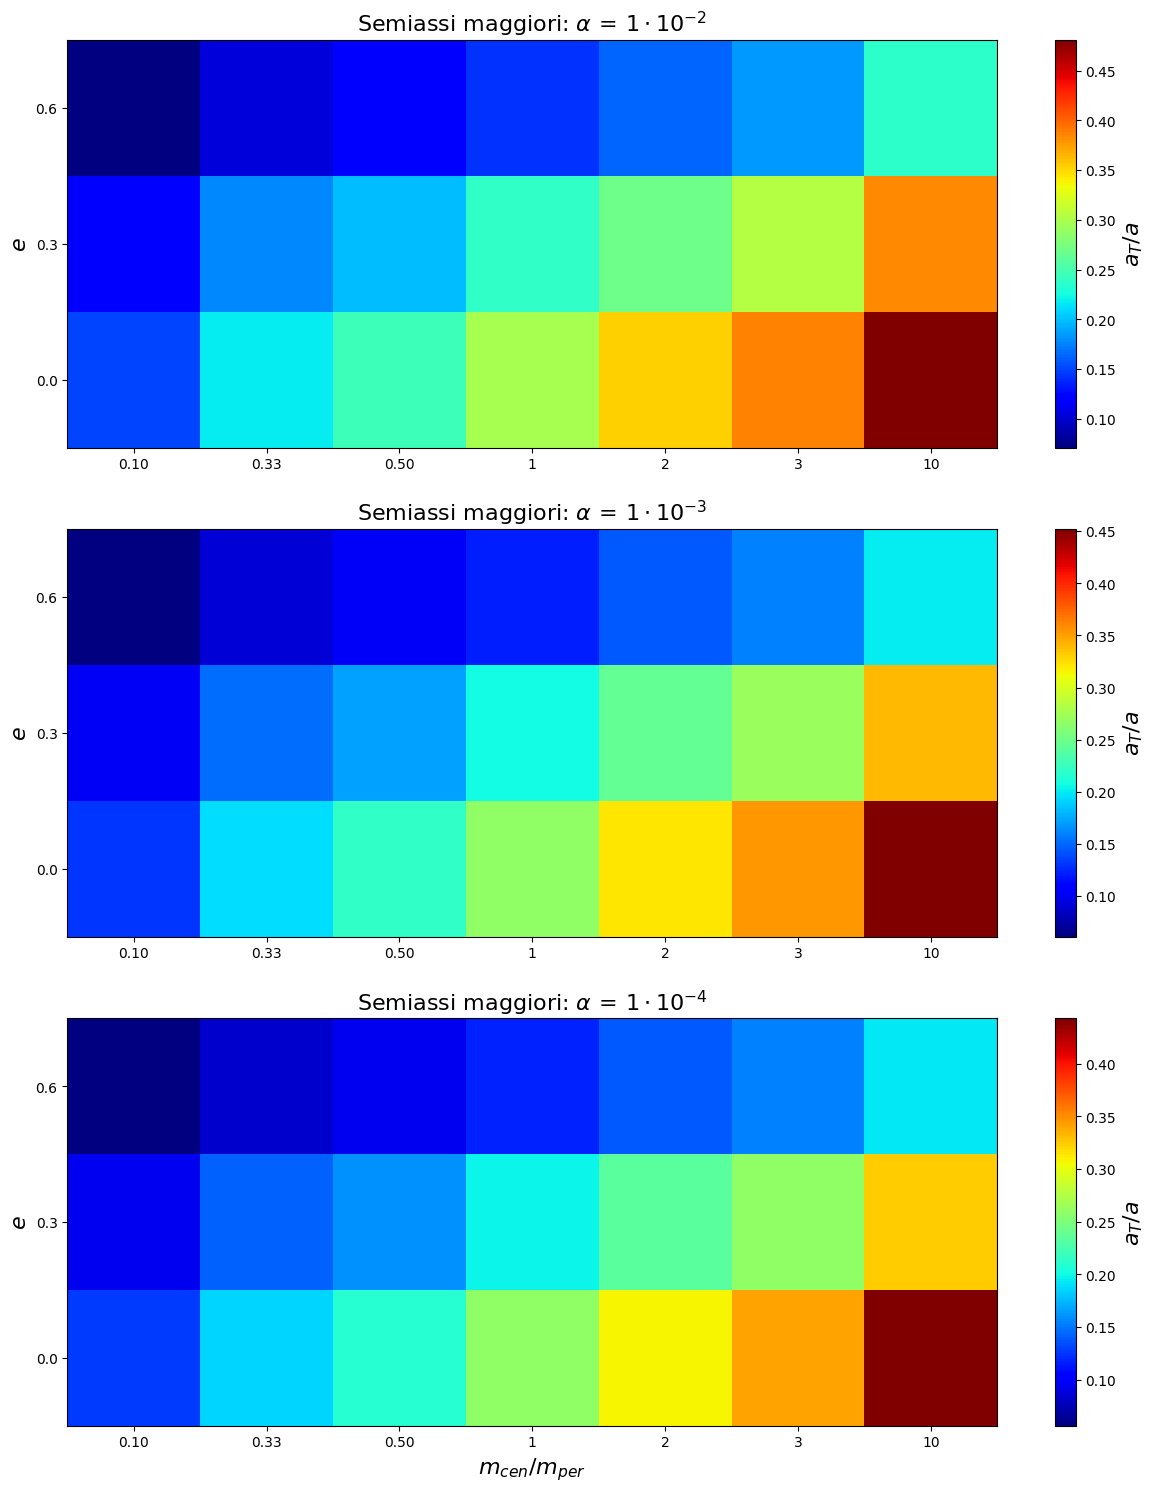
\includegraphics[width=\textwidth]{Immagini/graf_riass.png}
    \caption{In figura sono riportati i risultati ottenuti per i semiassi maggiori dei dischi: ogni grafico è dedicato ad un valore differente di $\alpha$. Sulle ascisse è posto il rapporto $m_{cen}/m_{per}$, dove $m_{cen}$ è la massa posta al centro della griglia, mentre $m_{per}$ quella del corpo perturbante. Notiamo come ad eccentricità della binaria fissata i dischi sono più grandi maggiore è la frazione di massa del sistema binario attorno alla quale orbitano. A $m_{cen}/m_{per}$ fissato, si può osservare una netta diminuzione delle dimensioni del disco all'aumentare di $e$.}
    \label{fig:sax_magg}
\end{figure}

Osserviamo che ad $e$ fissato, la dimensione del disco dipende fortemente dal valore di $m_{cen}/m_{per}$, dove $m_{cen}$ è la massa della stella al centro della griglia, mentre $m_{per}$ la massa del corpo perturbante: i dischi che orbitano attorno ad una frazione di massa della binaria più elevata sono più grandi.
All'aumentare di $e$ le dimensioni dei dischi circumstellari analizzati diminuiscono sensibilmente: questo andamento è dovuto al fatto che le risonanze eccentriche sono di intensità maggiore per un sistema altamente eccentrico, con un conseguente spostamento della regione di troncamento \parencite{ArtymowiczLubow1994}.
\'E possibile osservare una dipendenza da $\alpha$: maggiore è la viscosità, maggiori sono le dimensioni del disco che otteniamo.

Per le estensioni dei dischi abbiamo effettuato un confronto con i valori noti presenti in letteratura.
\cite{ManaraTronc2019} hanno proposto una formula analitica per la determinazione del raggio di troncamento
\begin{equation}
r_t\,=\,R_{L} (\alpha e^\beta\,+\,\gamma\mu^\delta),
\label{eq:tronc_disc}
\end{equation}
dove $R_L$ è la dimensione spaziale del Roche-Lobe \parencite{Eggleton1983}, $\gamma\,=\,0.88$ e $\delta\,=\,0.01$ sono dei parametri determinati fittando i risultati ottenuti da \cite{PapaloizouPringle1977} ed $\alpha$, $\beta$ sono stati calcolati fittando i risultati numerici ottenuti da \cite{ArtymowiczLubow1994}.
Abbiamo osservato una buon accordo con i valori noti in letteratura nei sistemi binari mediamente eccentrici od altamente eccentrici: nel caso di $e\,=\,0.0$ la teoria descrive correttamente il modo di scalare delle dimensioni del disco in dipendenza di $m_2/m_1$, ma sono presenti discrepanze del $15/20\,\%$ fra valori teorici e valori simulati.
Considerata la robustezza del codice FARGO3D, uno dei possibili sviluppi futuri di questo lavoro di tesi potrebbe essere un nuovo fit dei parametri $\alpha,\,\beta,\,\gamma,\,\delta$ individuati da \cite{ManaraTronc2019}.

\end{document}
